% !TeX spellcheck = en_US
\chapter{\iceact Simulation}\label{chap:iceact_sim}

This chapter will discuss the \geant simulation process. \todo{bisschen mehr?}

\section{Simulation of Single Components}

In order to make some first checks and optimization, the focus is on single essential components, i.e. the Fresnel lens and the Winston cones.

\subsection{\enquote{Best} Wavelength}

Many of the \iceact telescope properties have (non-linear) wavelength dependencies (cf. section~\ref{sec:iceact:model:material}). Additionally, the Cherenkov spectrum is wavelength dependent as well (cf. figure~\ref{airshowers:cherenkovspectrum}). By implication, there has to be a wavelength $\lambda^\ast$ that \iceact is the most efficient. One can determine $\lambda^\ast$ by looking at the following limiting functions.

\begin{itemize}
	\item The Cherenkov spectrum. The data shown in figure~\ref{airshowers:cherenkovspectrum} (La Palma, \SI{2200}{\meter} a.s.l.) is chosen.
	\item The internal transmission function of PMMA. It is assumed that a photon has to pass approximately \SI{30}{\milli\meter} of PMMA to get to the SiPMs. Thus, the internal transmission function shown in figure~\ref{iceact:model:material:transmission} as blue dotted-dashed line has to be exponentiated by \num{10} to hold for this case.
	\item The internal transmission function of borosilicate, i.e. the material of the glass plate. The photons have to pass approximately \SI{2}{\milli\meter}. Exponentiation of a factor $\frac{2}{3}$ of the orange dotted-dashed line in figure~\ref{iceact:model:material:transmission} leads to the desired function.
	\item The photon detection efficiency (PDE) function of the SiPMs interpolated for $V_\text{OV} = \SI{5}{\volt}$ (cf. orange curve in figure~\ref{sipm:pde}).
\end{itemize}

All of these functions are normalized, i.e. divided by their own maximum, and than multiplied which results in a new (relative) efficiency function. The maximum of this function again is the \enquote{best} wavelength found to be $\lambda^\ast = \SI{411}{\nano\meter}$. Figure~\ref{best_wvl} shows the procedure graphically. 

\begin{figure}[H]
	\centering
	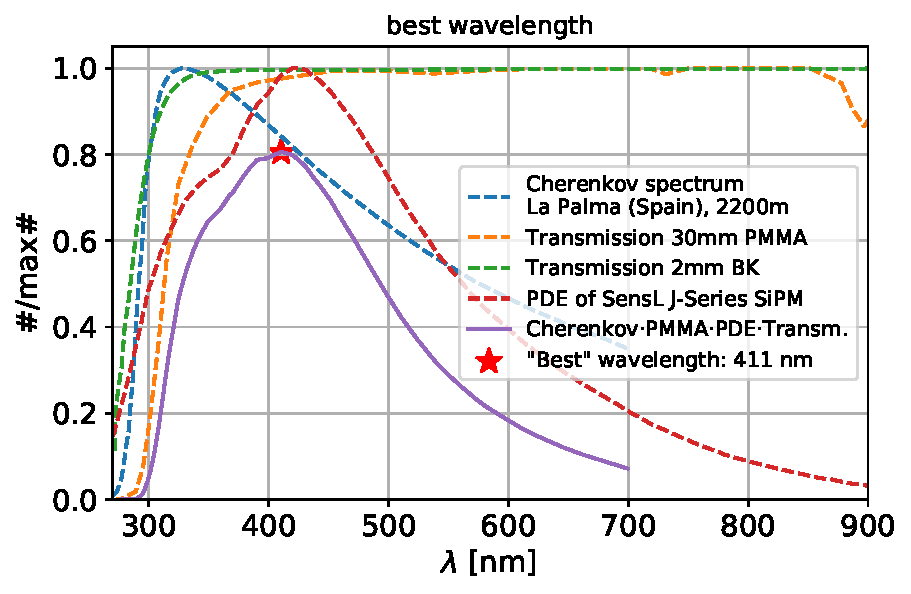
\includegraphics[width=0.7\textwidth]{best_wvl.pdf}
	\caption[\enquote{Best} wavelength]{\textbf{\enquote{Best} wavelength.} All limiting functions (Cherenkov spectrum, matrial transmission curves, and photon detection efficiency) are nomalized to each maximum and multiplied. The maximum of the product is defined to be the \enquote{best}, i.e. most efficient, wavelength $\lambda^\ast=\SI{411}{\nano\meter}$.}
	\label{best_wvl}
\end{figure}

\subsection{Focal Plane Shift}

\begin{figure}[H]
	\centering
	\begin{subfigure}[t]{0.49\textwidth}
		\centering
		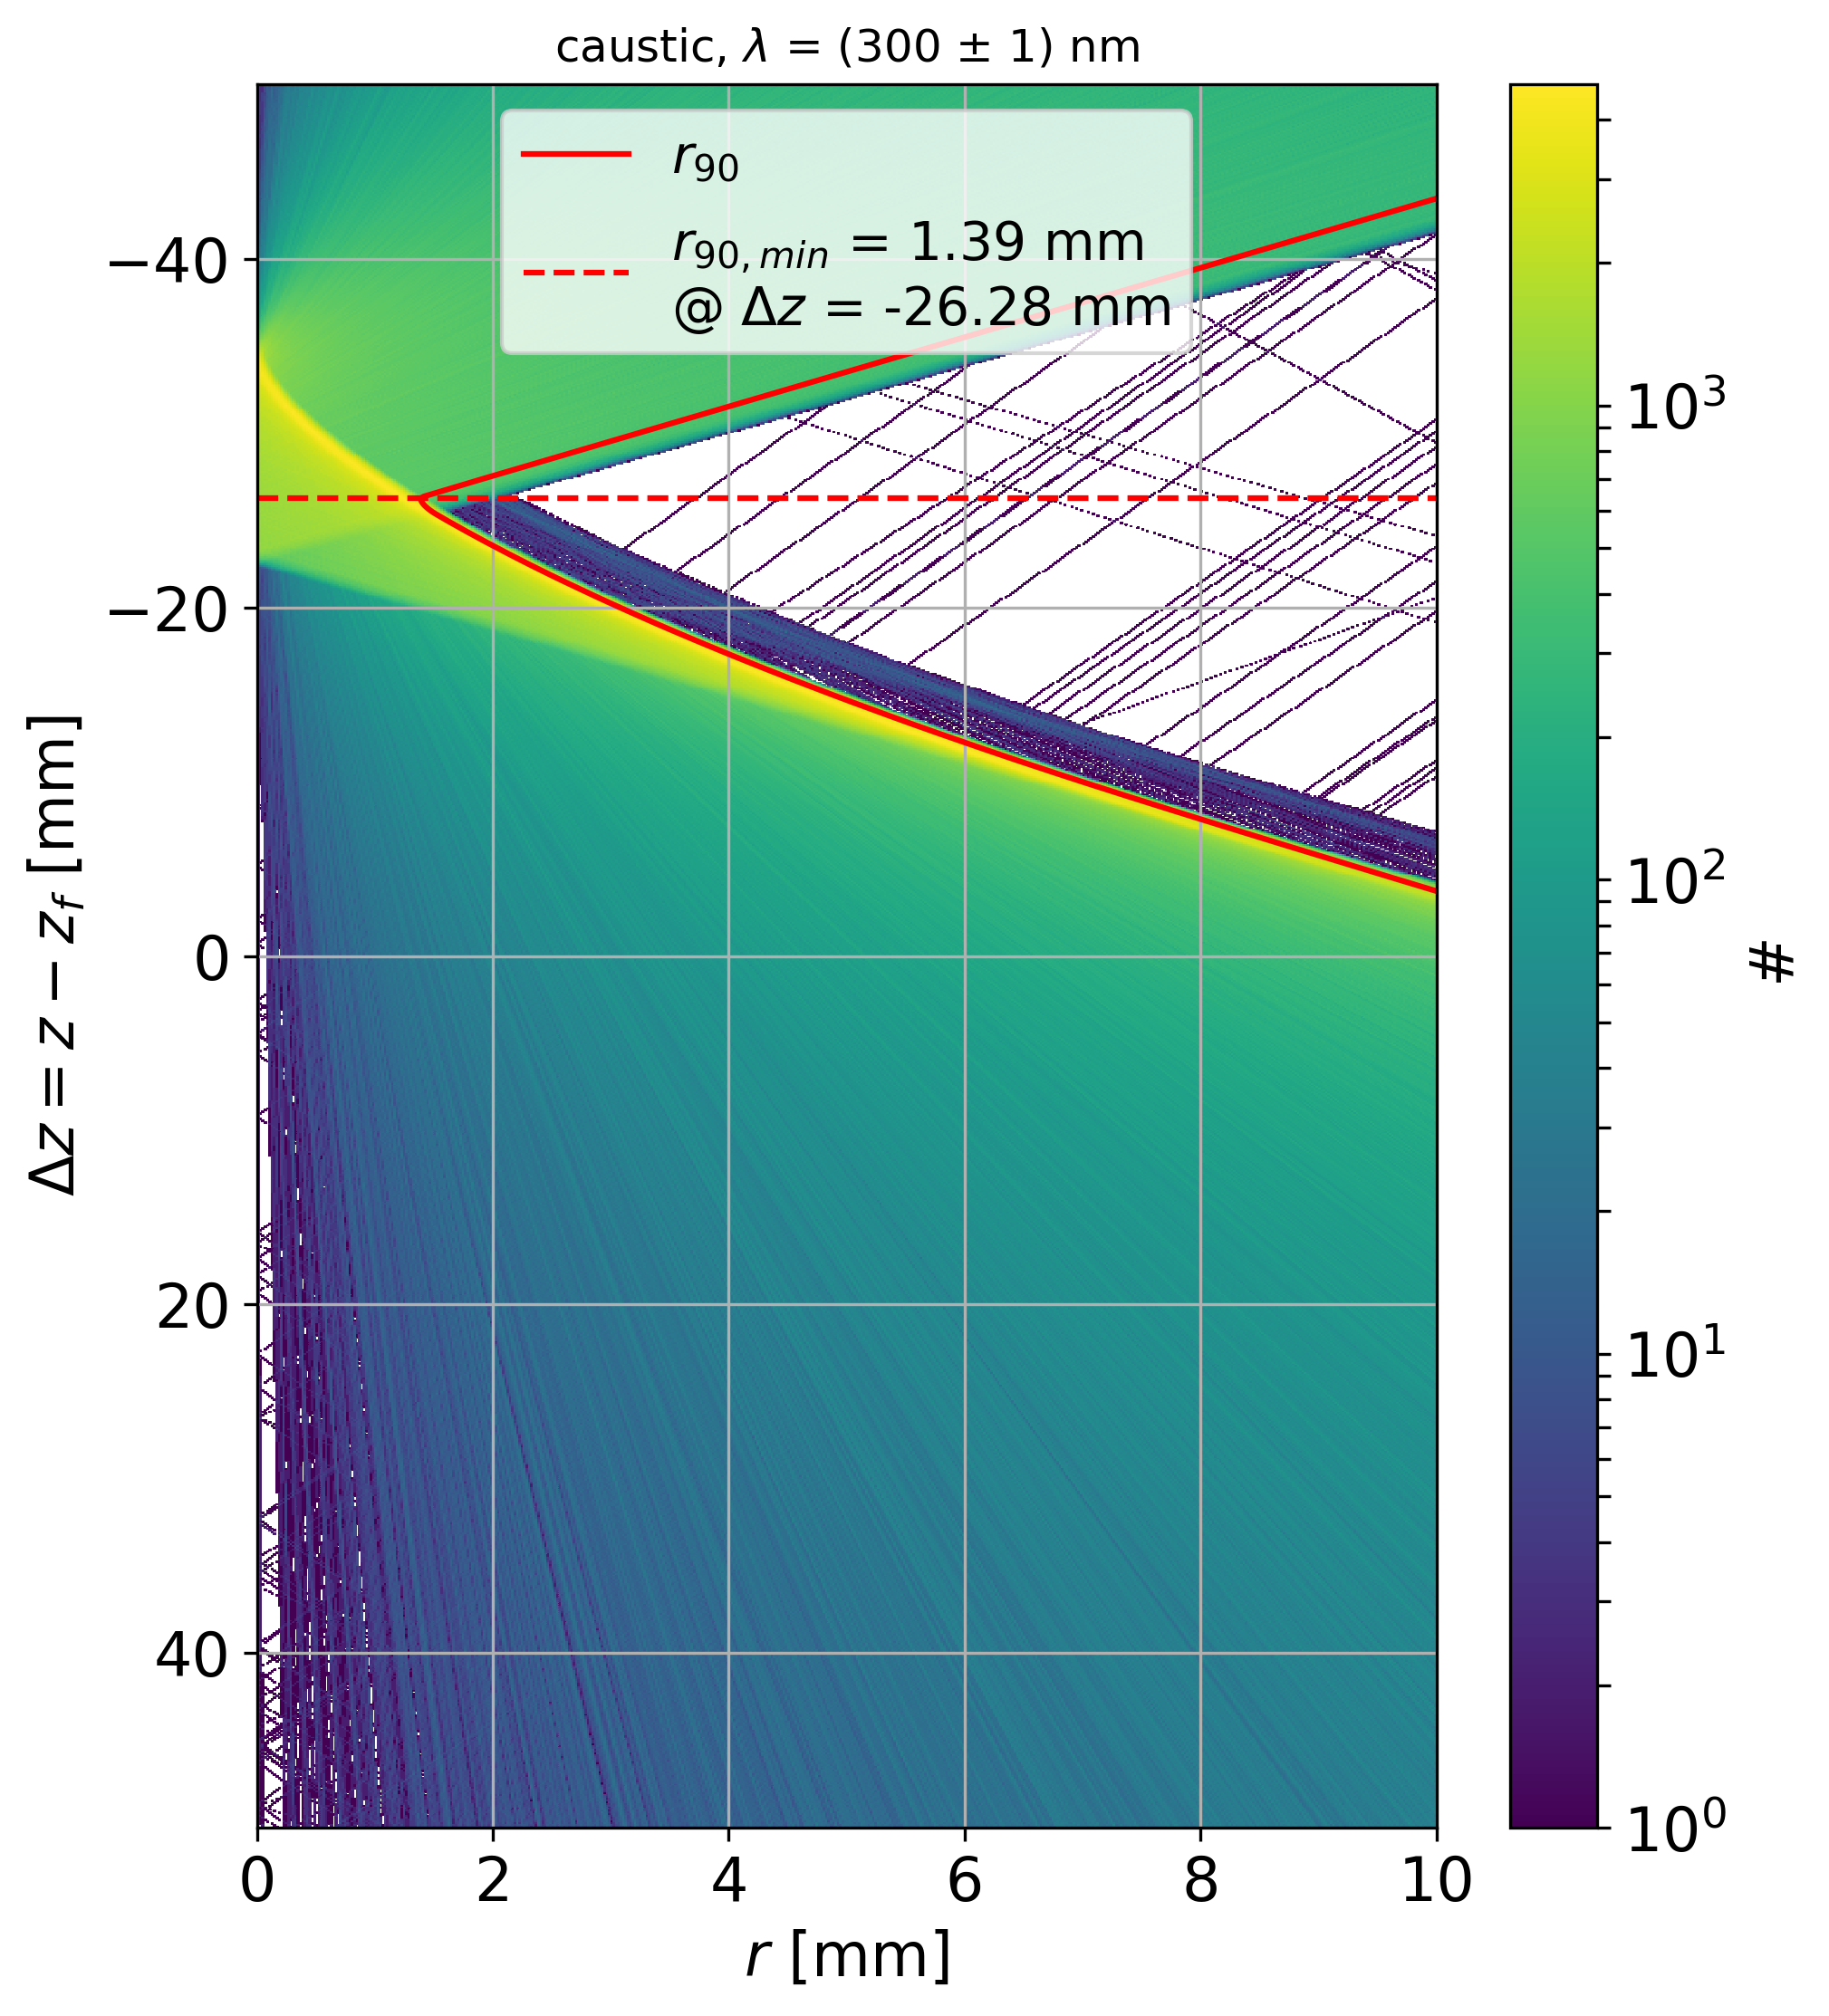
\includegraphics[width=\textwidth]{focalplaneshift/caustic_300nm.png}
		\subcaption{}
	\end{subfigure}
	\hfill
	\begin{subfigure}[t]{0.49\textwidth}
		\centering
		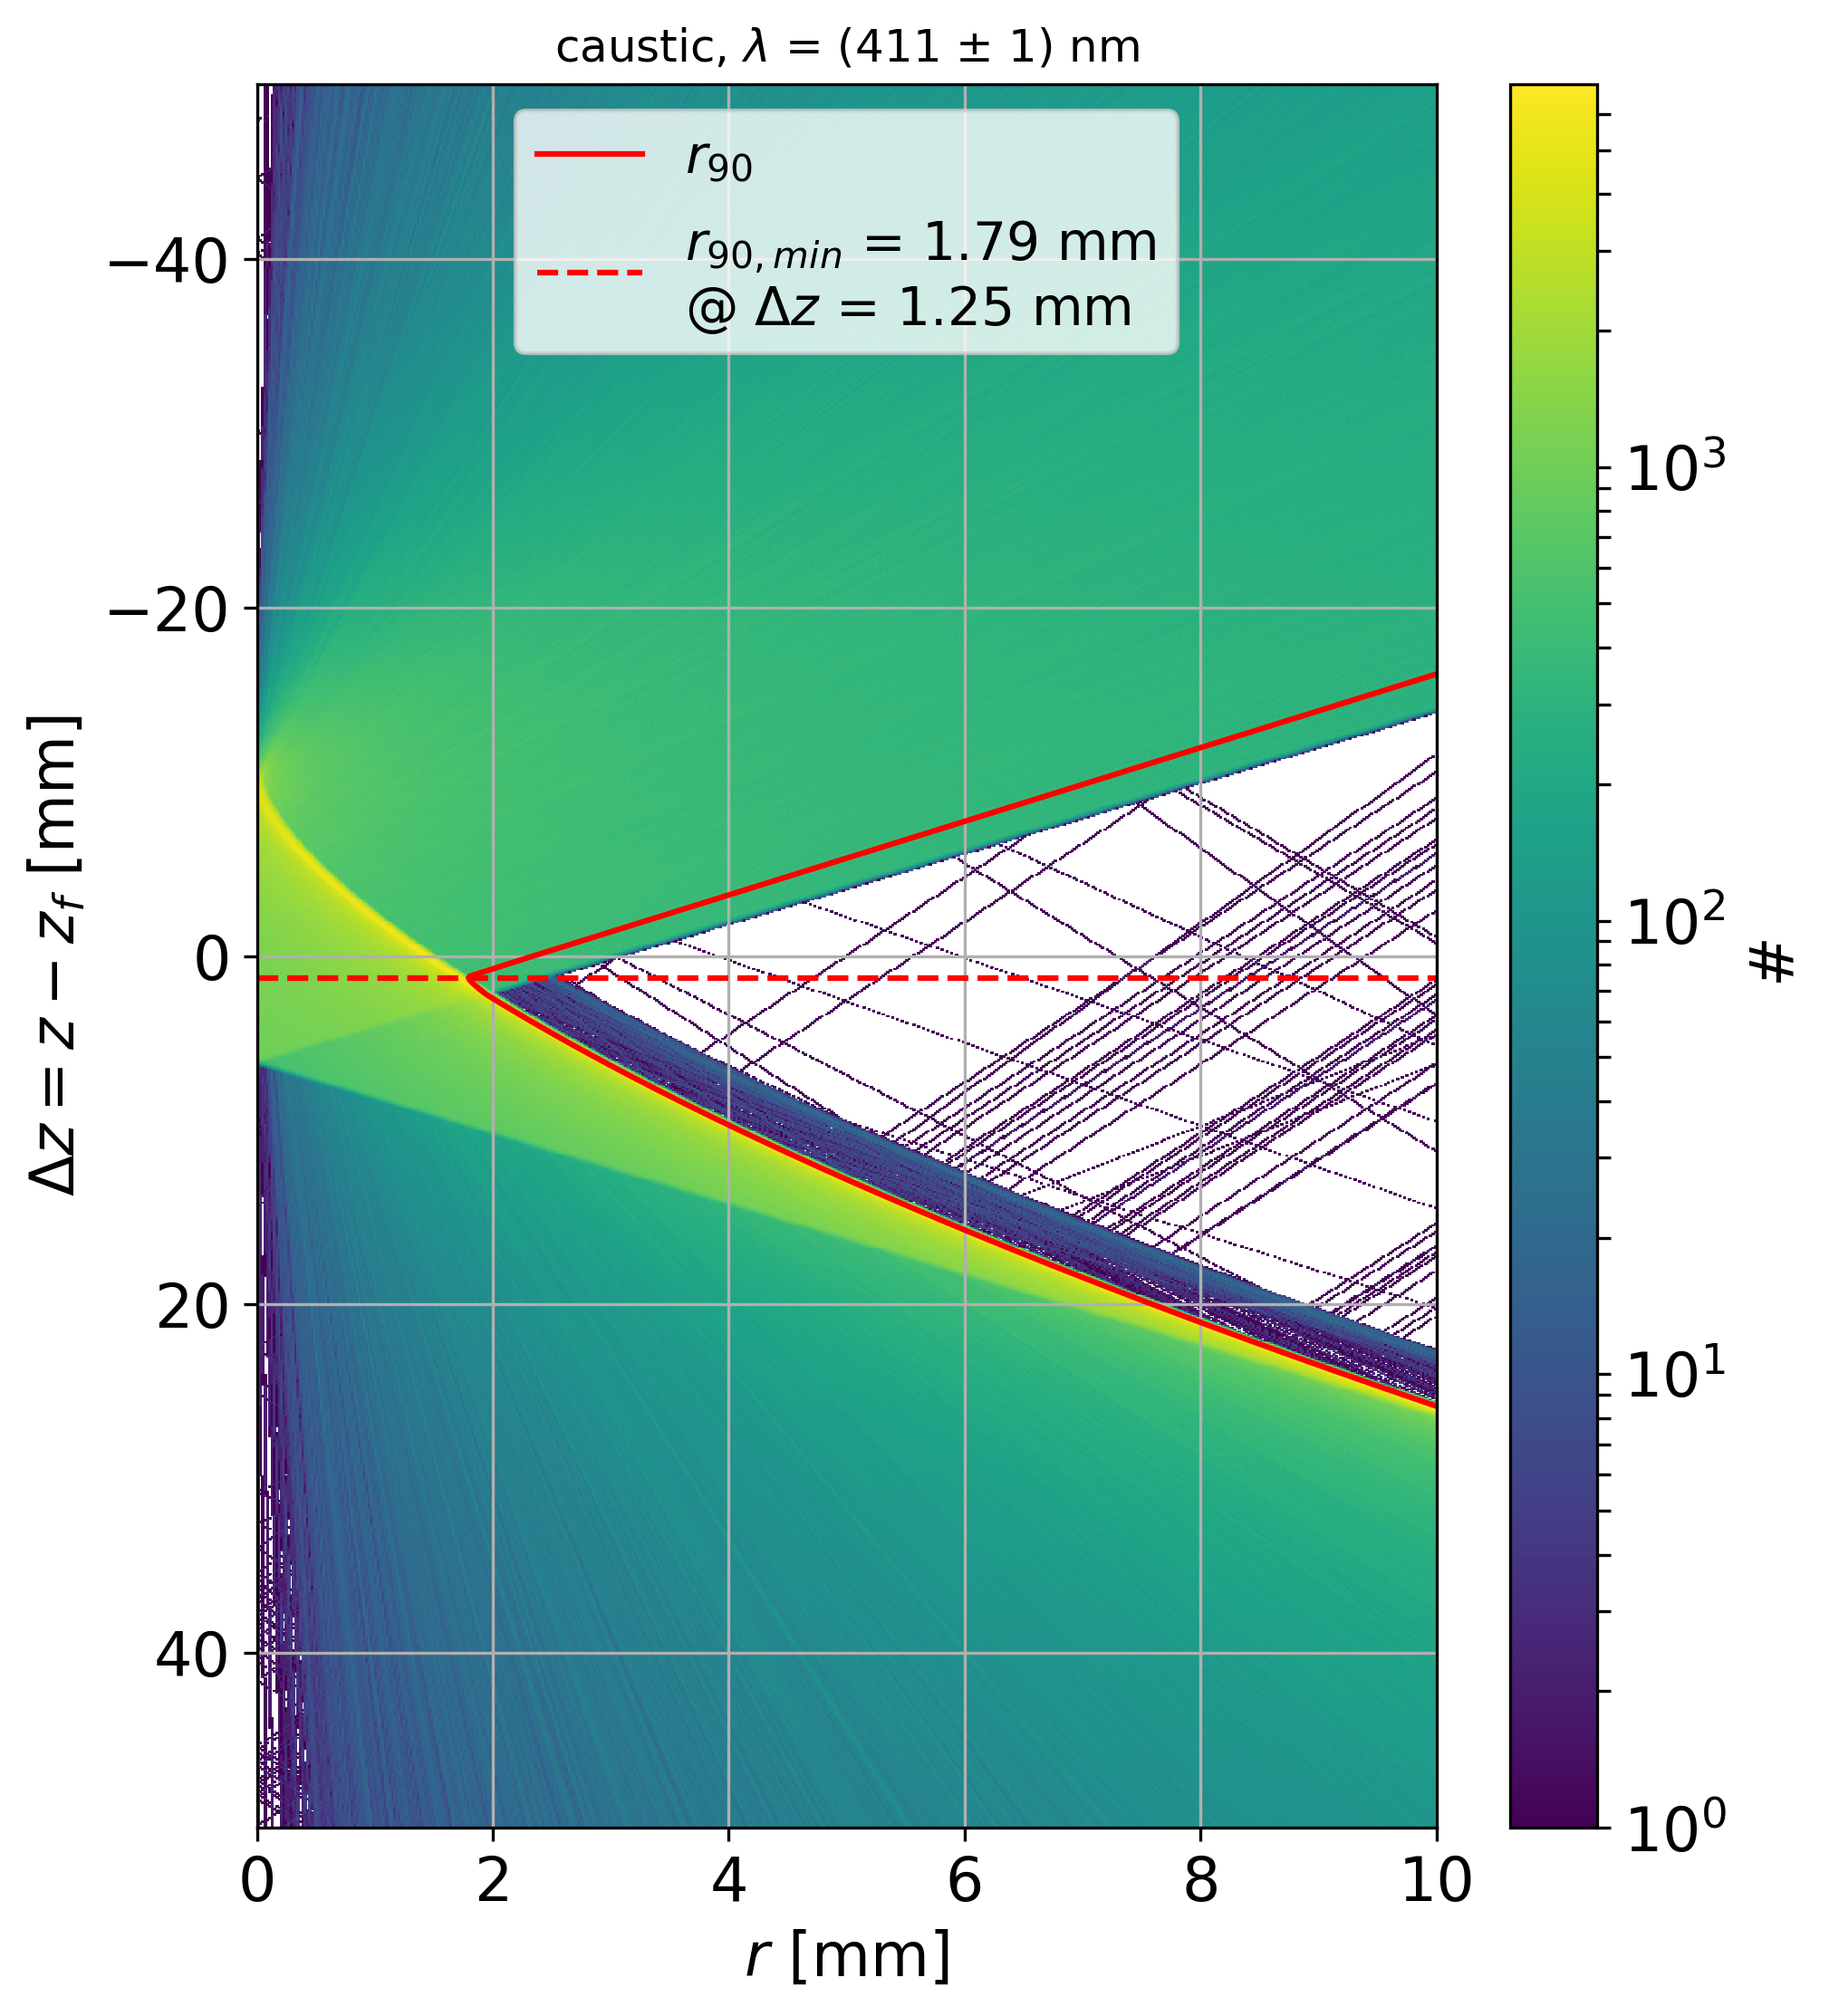
\includegraphics[width=\textwidth]{focalplaneshift/caustic_411nm.png}
		\subcaption{}
		\label{focalplaneshift_bestwvl}
	\end{subfigure}
	\hfill
	\begin{subfigure}[t]{0.49\textwidth}
		\centering
		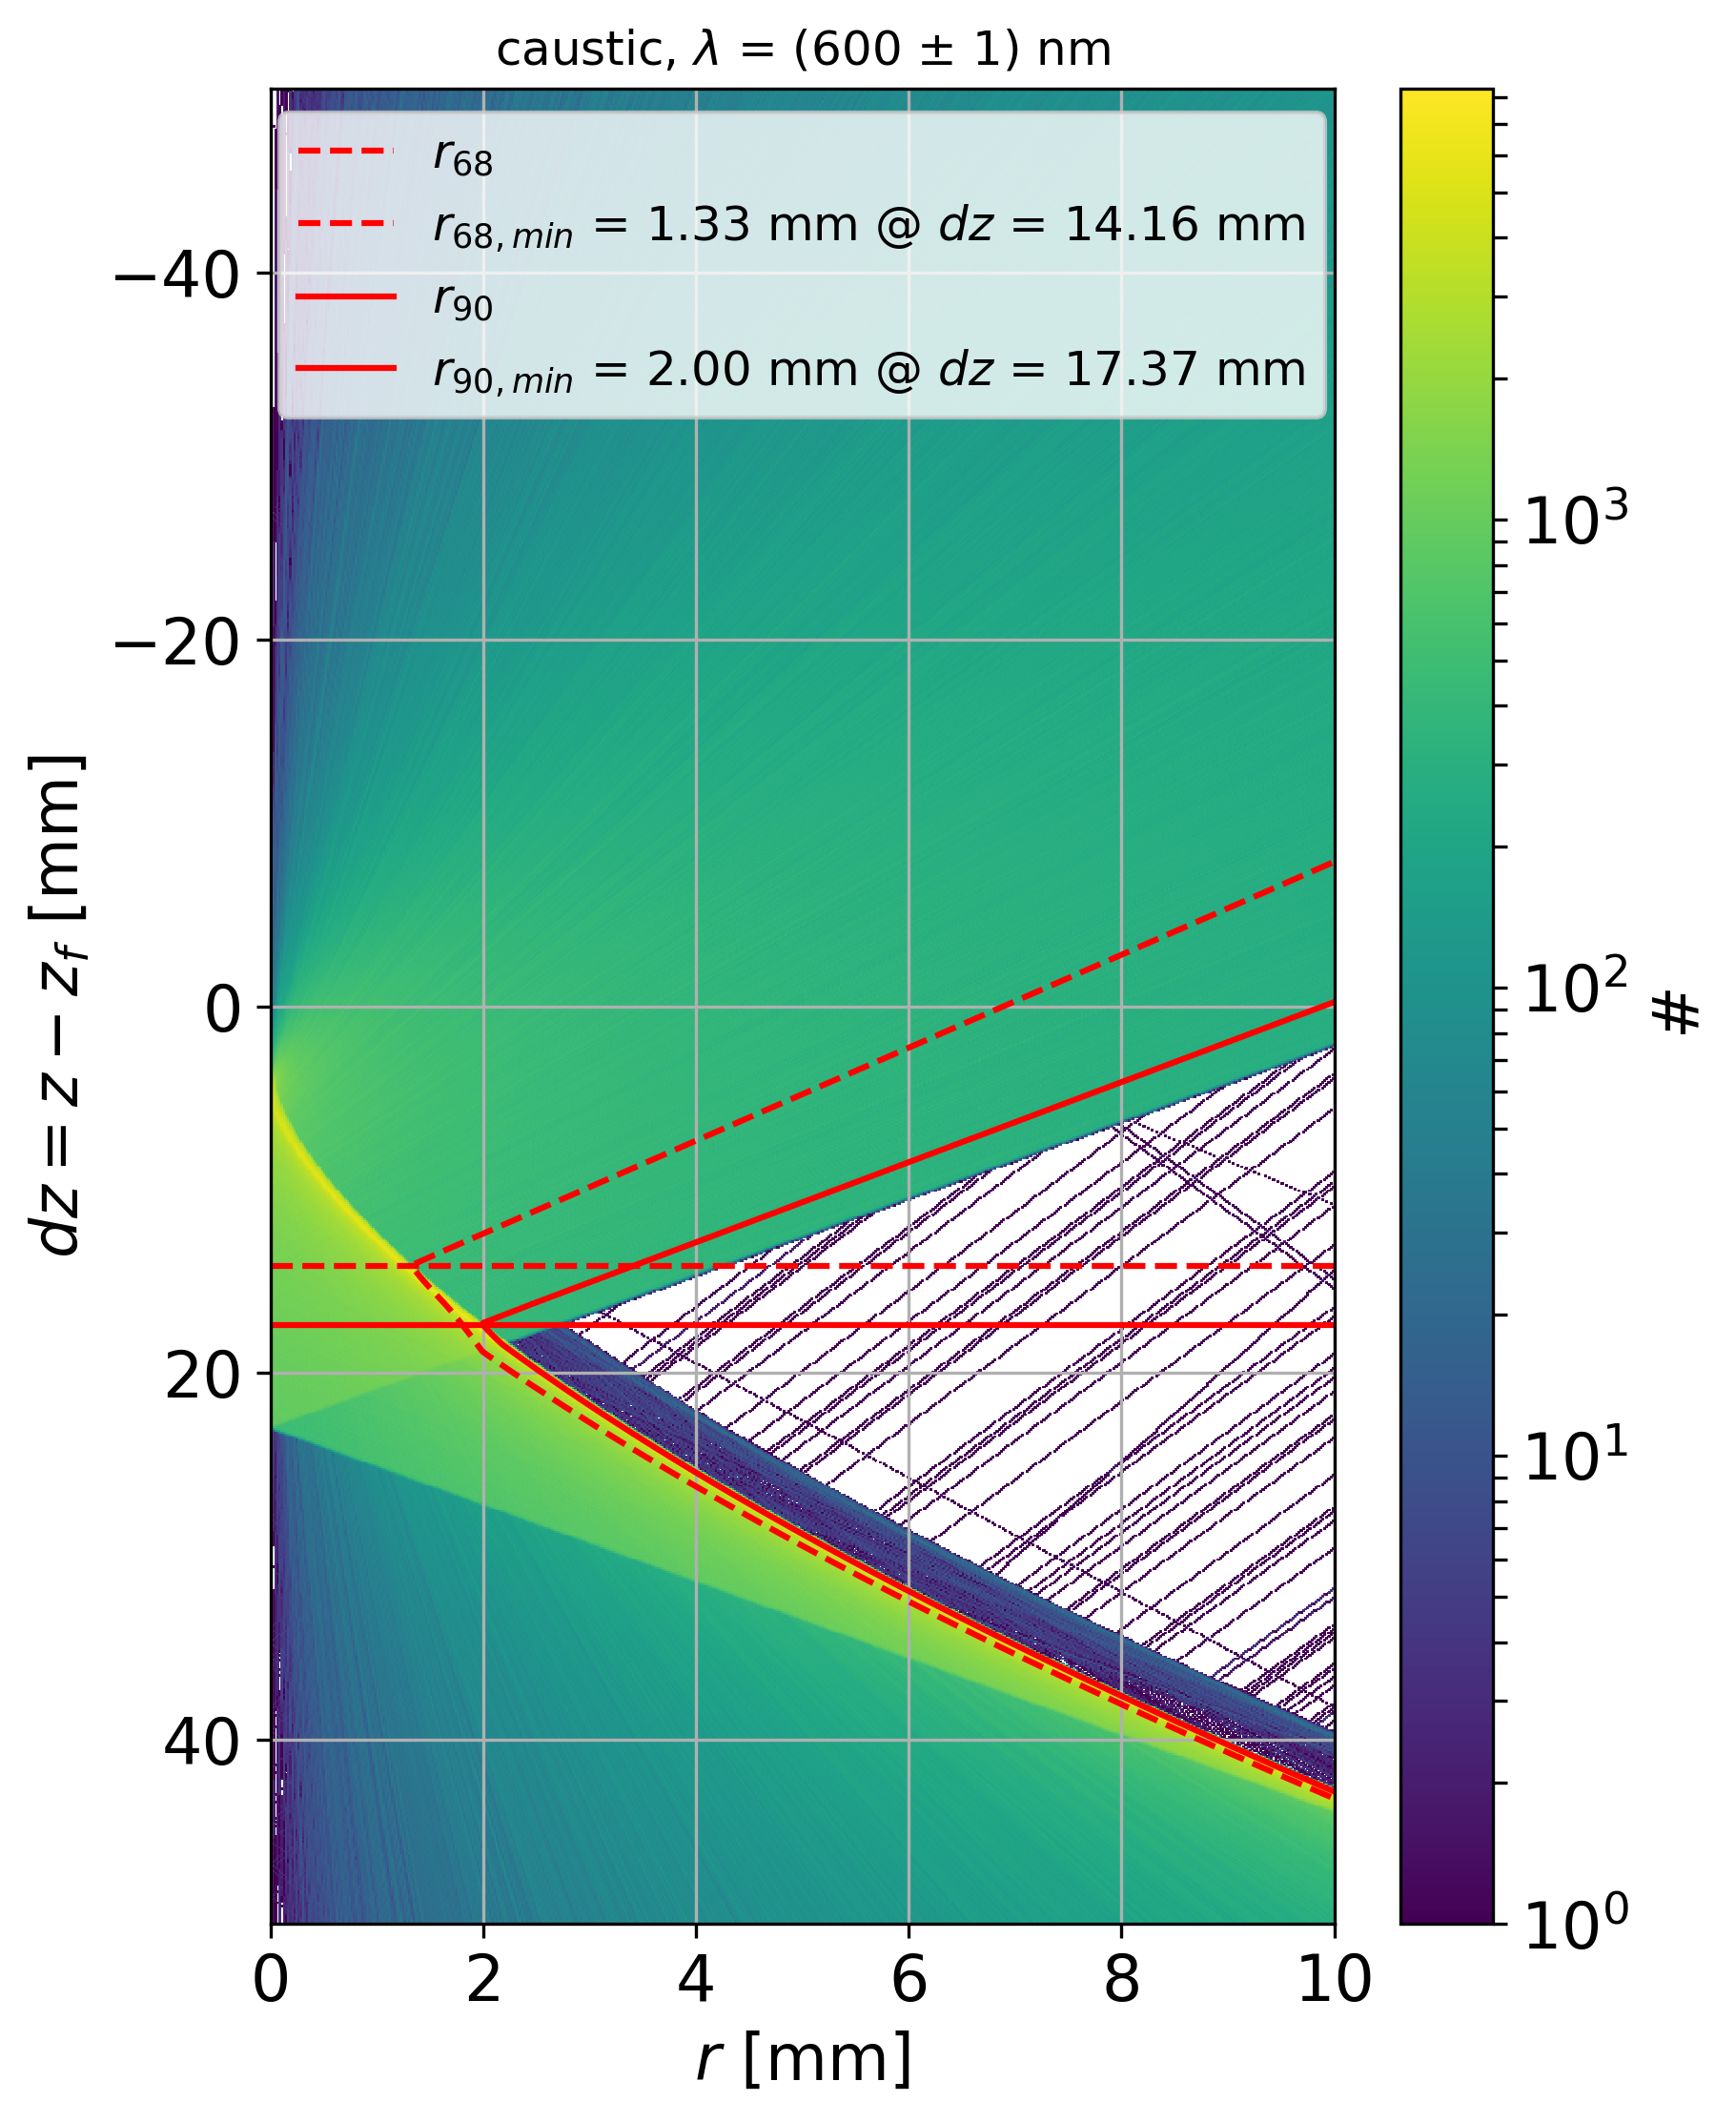
\includegraphics[width=\textwidth]{focalplaneshift/caustic_600nm.png}
		\subcaption{}
	\end{subfigure}
	\hfill
	\begin{subfigure}[t]{0.49\textwidth}
		\centering
		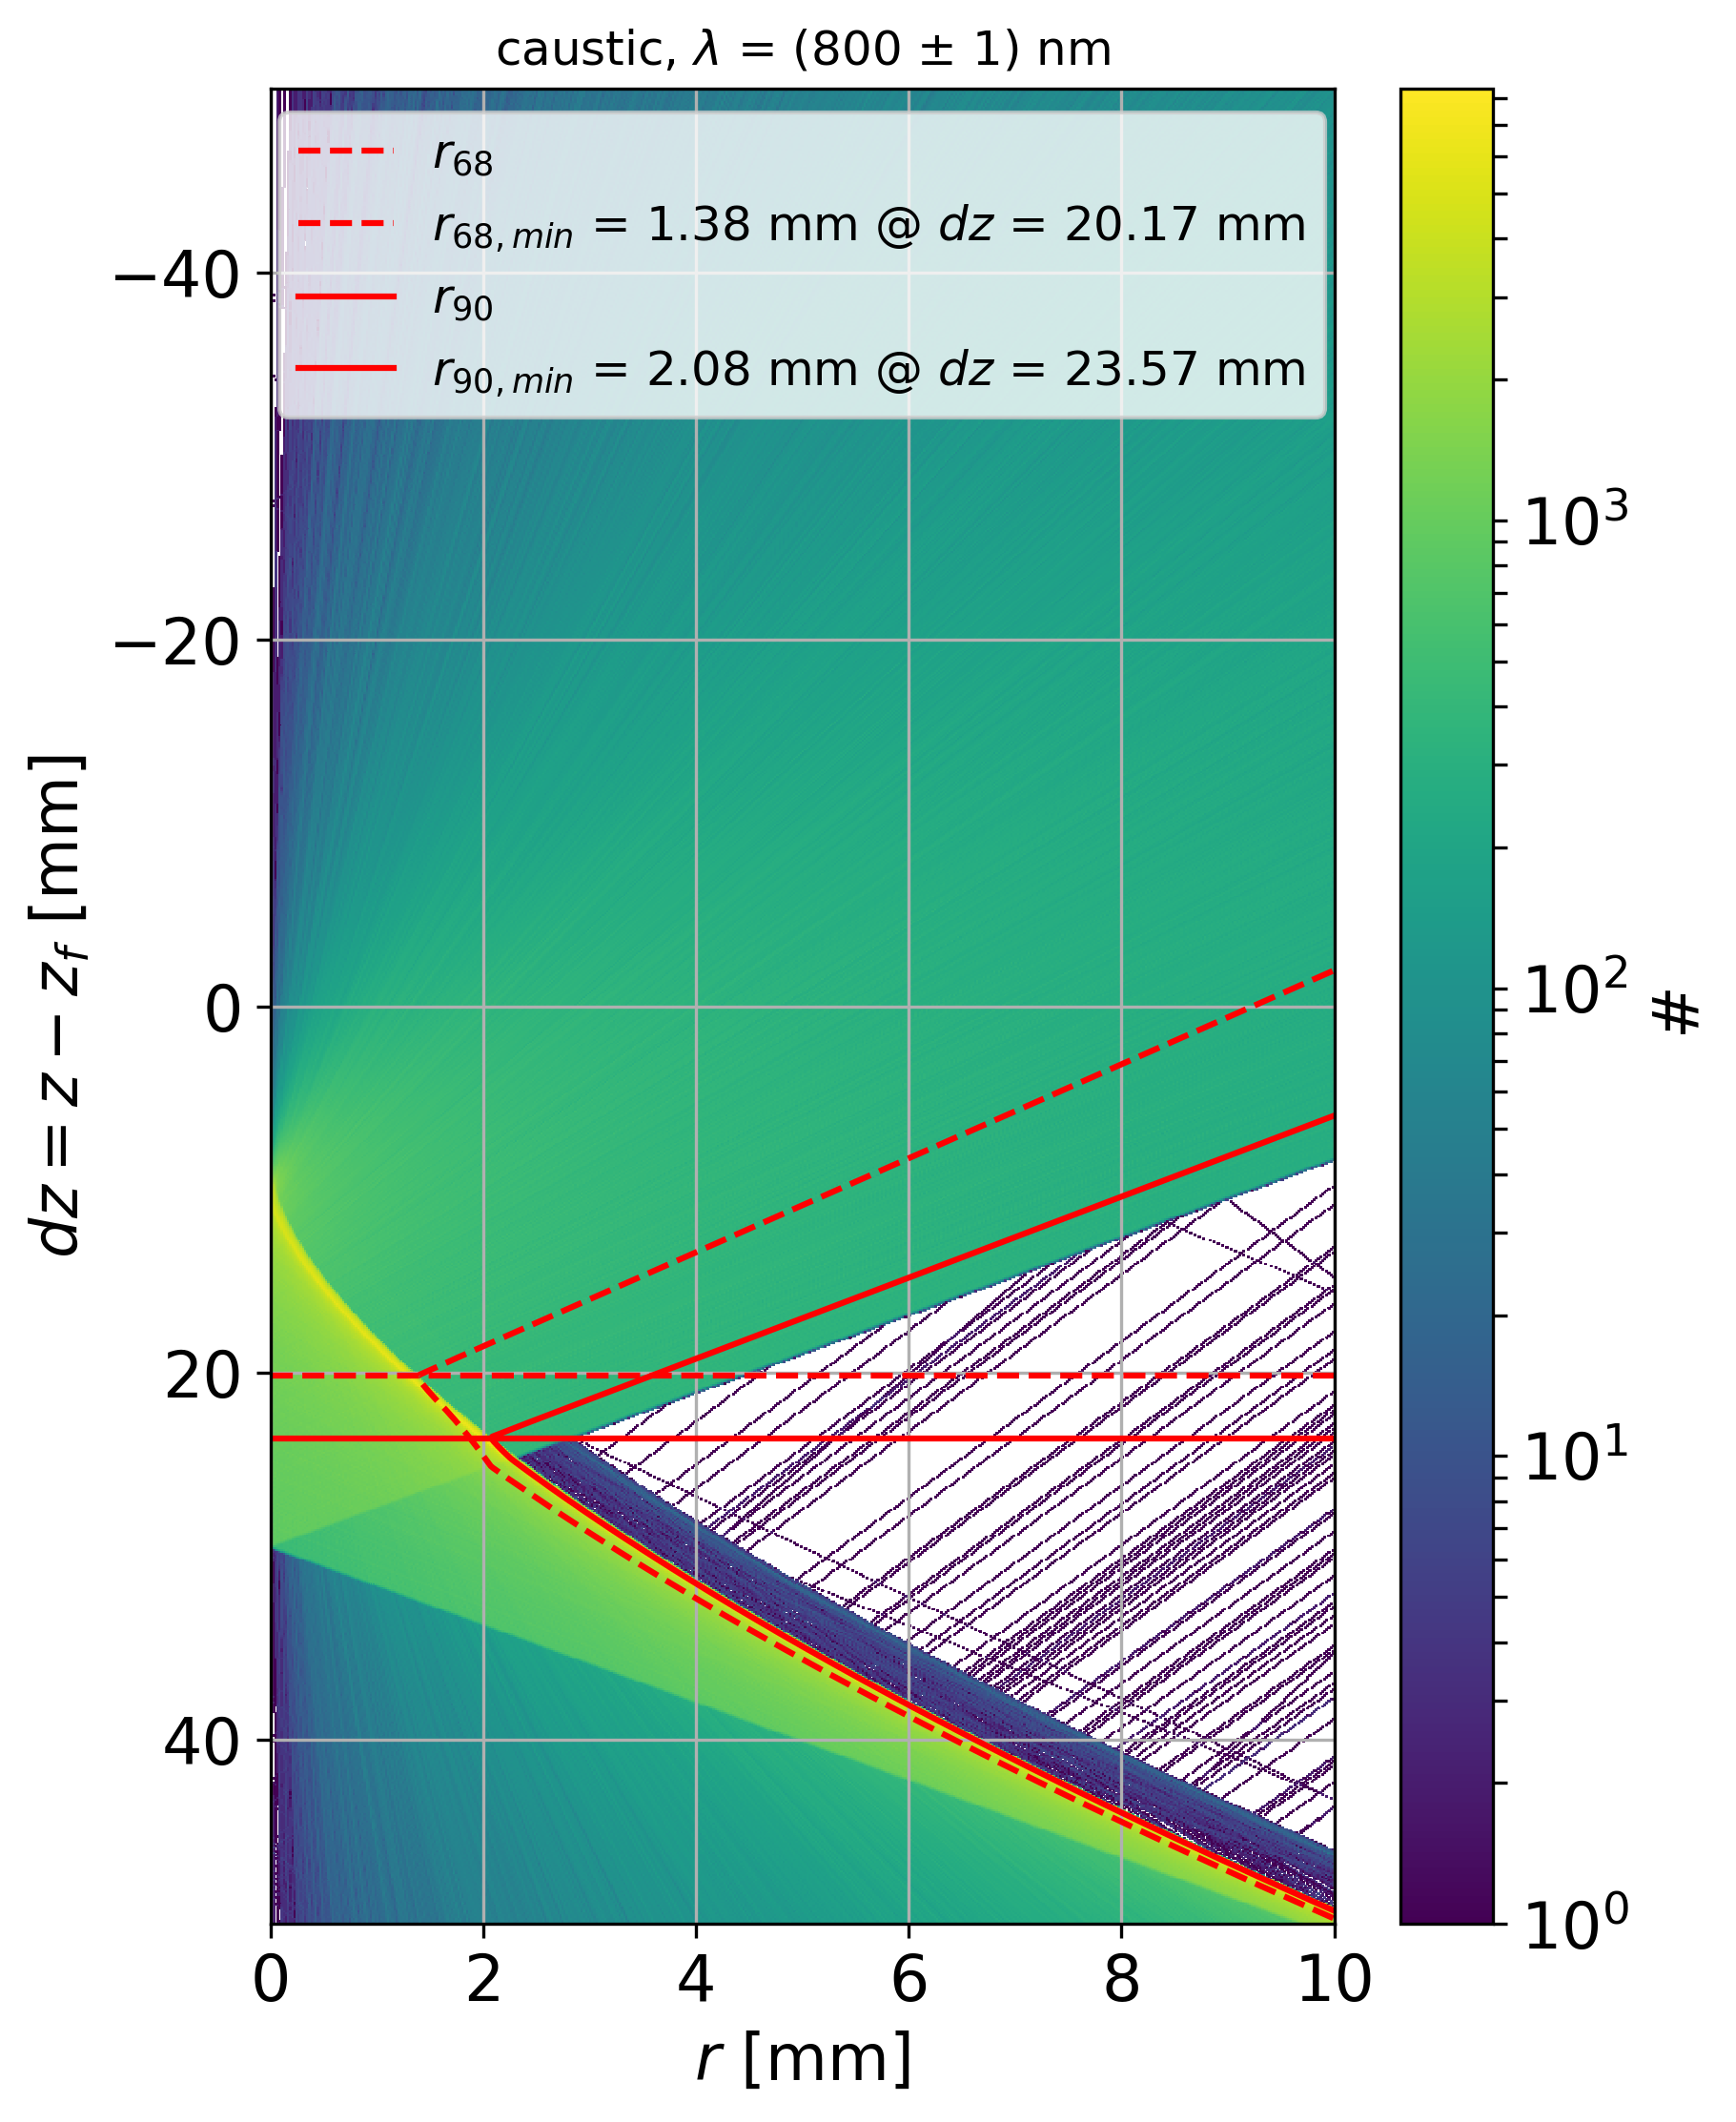
\includegraphics[width=\textwidth]{focalplaneshift/caustic_800nm.png}
		\subcaption{}
	\end{subfigure}
	\caption[]{}
	\label{focalplaneshift}
\end{figure}

\subsection{Winston Cone Simulation}

\section{Simulation Strategy and Verification}

\subsection{Winston Cone Meshing}\label{sec:wico_meshing}

\subsection{Aberration Effects -- \enquote{Ghost Image}}\label{sec:ghost_image}

\begin{figure}[H]
	\centering
	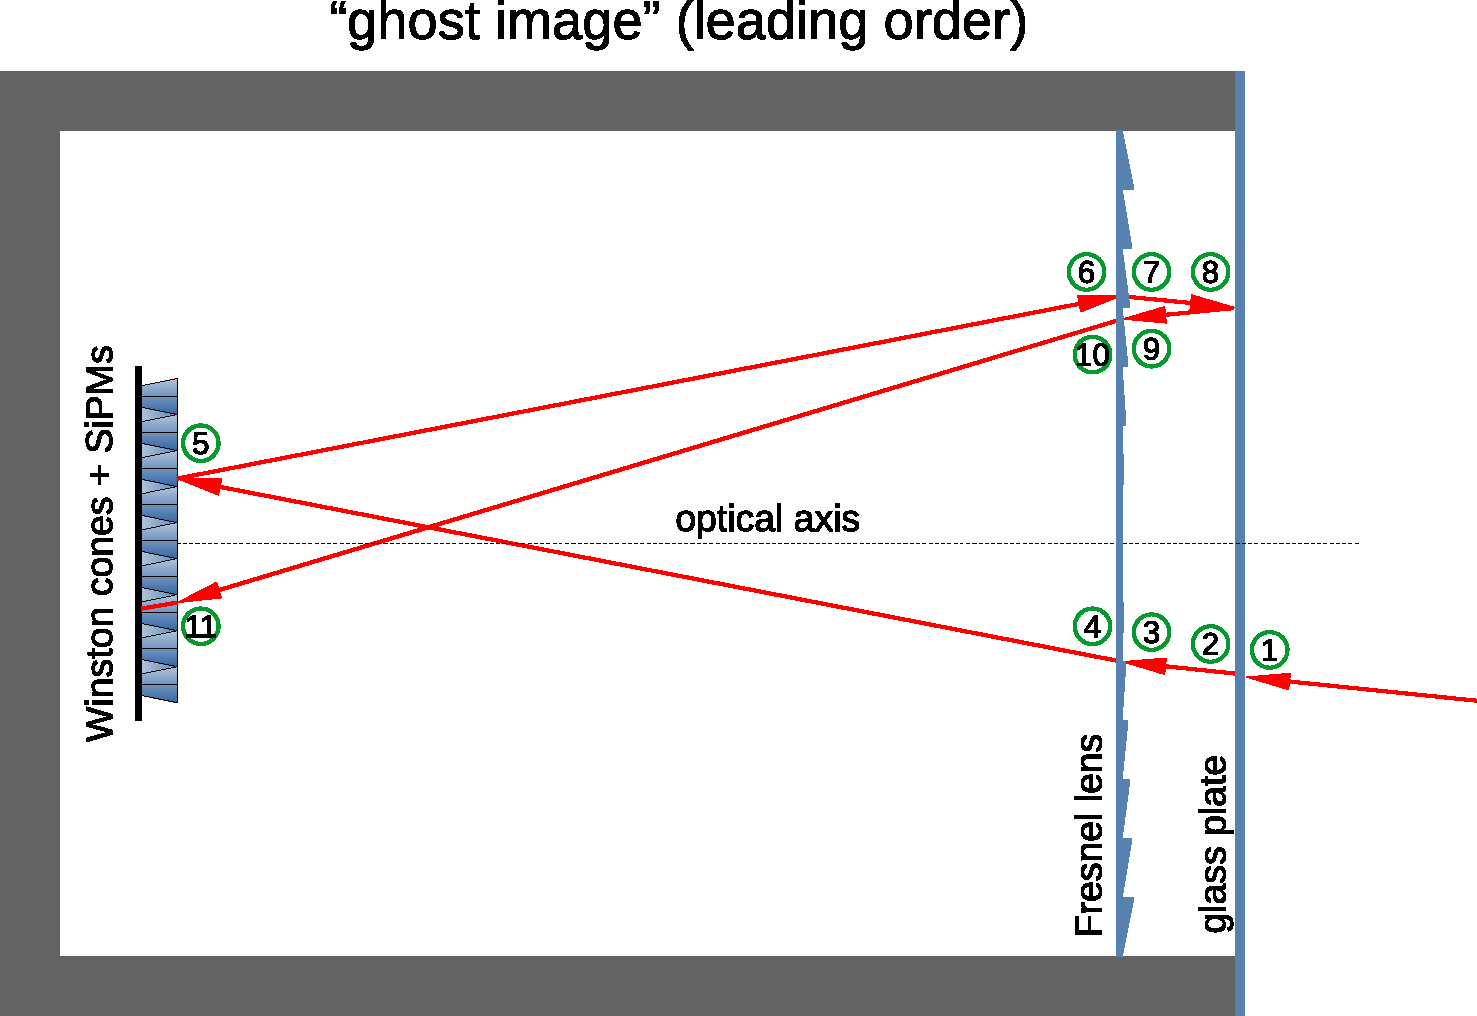
\includegraphics[width=0.9\textwidth]{GhostImage.pdf}
	\caption[Schematic sketch for the \enquote{ghost image} ray path]{\textbf{Schematic sketch for the \enquote{ghost image} ray path.} long caption}
	\label{ghostimage_path}
\end{figure}

\section{Parametrization Simulation}

\begin{figure}[H]
	\centering
	\saveimageheight[width=0.49\textwidth]{GeantCoords.pdf}
	\begin{subfigure}[t]{0.49\textwidth}
		\raiseimage[width=\textwidth]{CameraPixels.pdf}
		\subcaption{Top view of the \iceact camera with pixel numbering and coordinate system. The $z$-axis comes out of the drawing plane.}
	\end{subfigure}
	\hfill
	\begin{subfigure}[t]{0.49\textwidth}
		\usebox{\savedimage}
		\subcaption{Coordinate system for the \iceact telescope. The tube is sketched as a the blue cylinder. The coordinate origin is set as the center of the focal plane on the Winston cones' entrance windows. An exemplary incoming photon drawn as red line impinges on the glass plate under a zenith angle $\theta$ and an azimuth angle $\phi$.}
	\end{subfigure}
	\caption[Coordinate system used in \geant and for the simulation]{\textbf{Coordinate system used in \geant and for the simulation.} }
	\label{geant_coords}
\end{figure}